\section{Introduction}\label{intro}\sloppy
Data cleaning is widely recognized as a major challenge in almost all forms of data analytics~\cite{nytimes}. 
The research community is developing increasingly sophisticated learning-based methods for detecting and repairing errors in large datasets~\cite{dc, rekatsinas2017holoclean, DBLP:journals/pvldb/KrishnanWWFG16, DBLP:conf/sigmod/ChuIKW16, mudgal2018deep, doan2018toward}.
As complexity grows, so does the number of user-facing parameters.
The burden on the analyst is gradually shifting away from the design of hand-written data cleaning programs, to parameter tuning in a sequence of multiple such automated systems.
Therefore, there is a need for systems that automatically tune and optimize parameters in data transformation and cleaning pipelines.

A starting point is the recent work on systems for \emph{hyperparameter tuning} for machine learning~\cite{li2017hyperband, sparks2017keystoneml, baylor2017tfx, golovin2017google, liaw2018tune}.
These systems are alternatively described as ``black box'' search algorithms as they make few assumptions about the underlying structure of the parameter space---simply put, generality at the cost of runtime.
In machine learning, the objective of the search process is clear: the prediction error on a validation set gives an estimate of accuracy. 
In data cleaning, there is a chicken-and-egg problem, where accuracy is defined in terms of recovering the true values of cells in a database, but knowing the true values in advance would defeat the purpose of cleaning.
In practice, we often use a proxy for accuracy such as the satisfaction of integrity constraints, how well it fits a statistical model, or accuracy on gold standard data.
Given one of these proxy accuracy metrics, is black-box hyperparameter tuning sufficient for applications in data cleaning optimization?

\begin{figure}[t]
\centering
 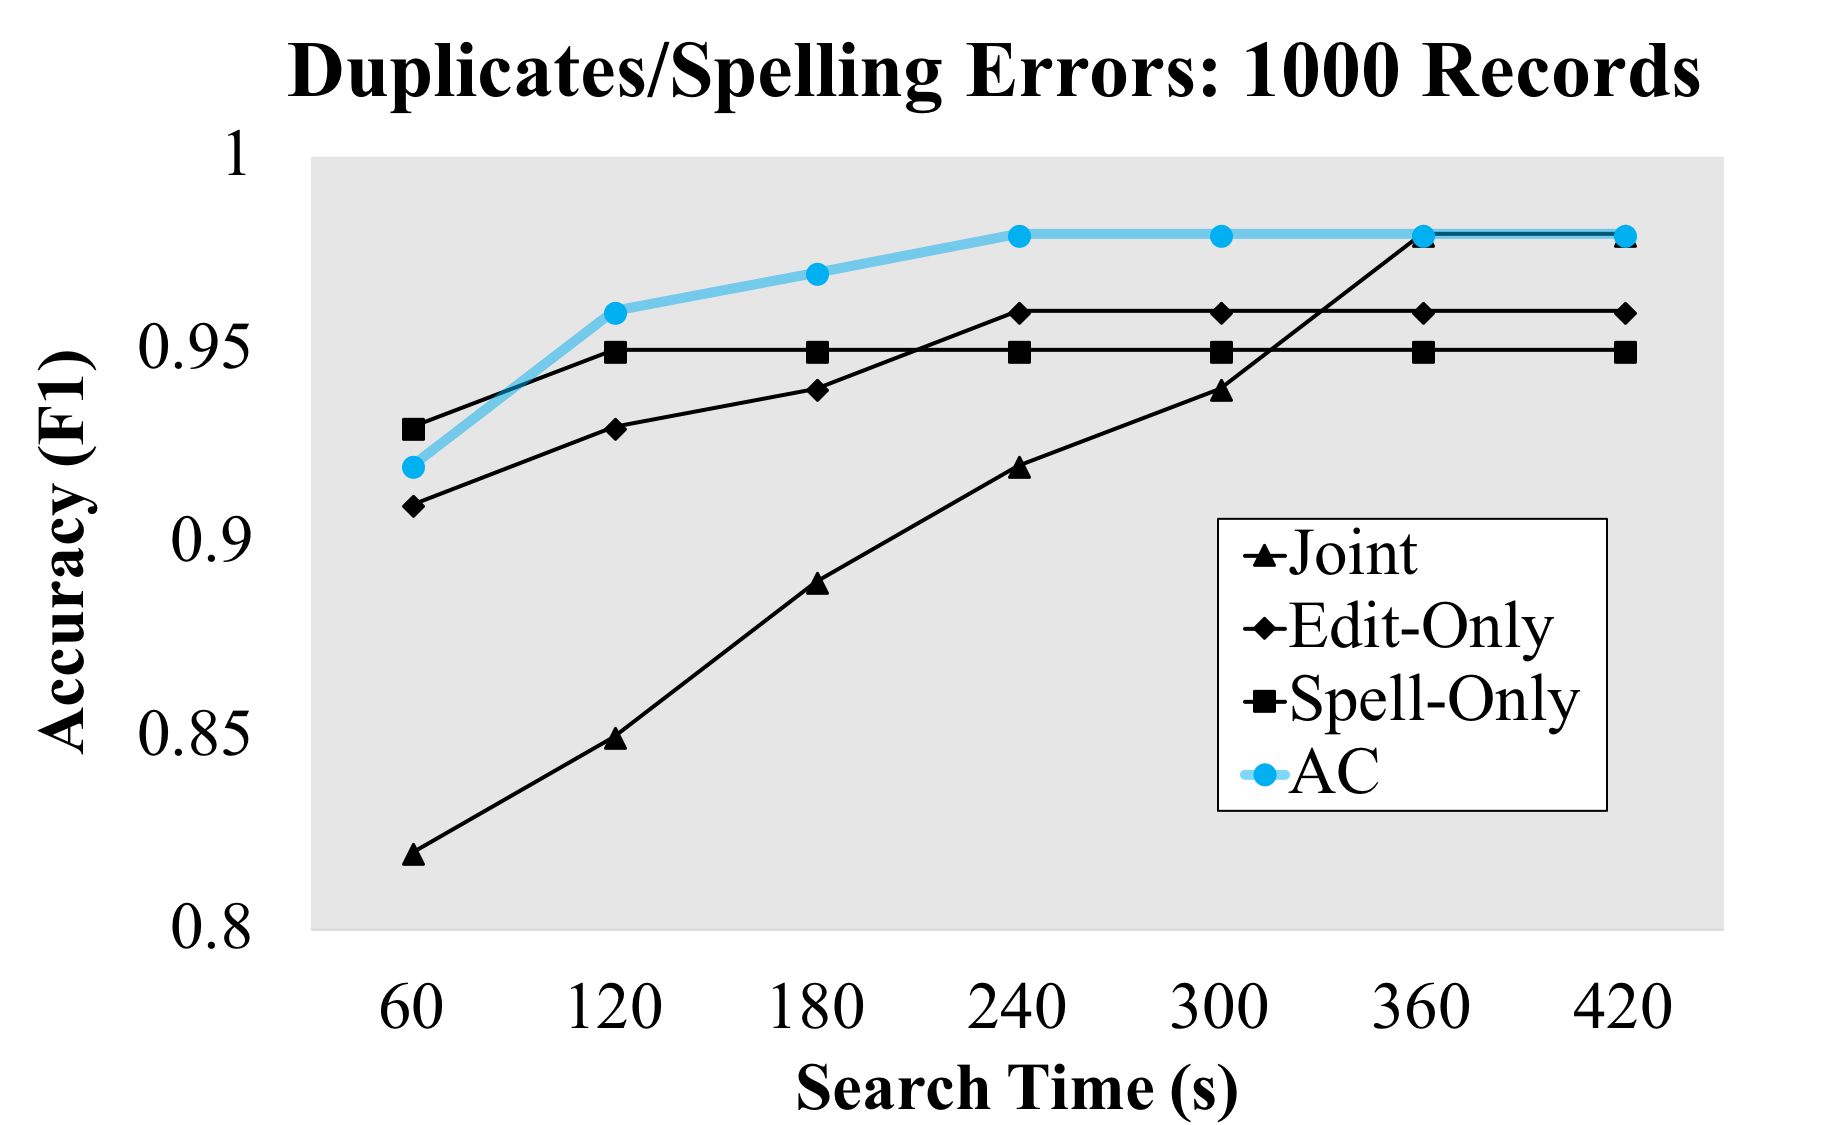
\includegraphics[width=0.9\columnwidth]{figures/teaser-experiment.png}
 \caption{\small 10\% of a dataset of dictionary words are duplicated with randomly generated spelling errors. The dataset is to be cleaned with a similarity matcher and a spell checker. Holistically, tuning the parameters of both with \textsf{python hyperopt} (Full) is inefficient due to interactions between the two data cleaning options. It takes over 3x the amount of search time for the joint optimization to exceed the best tuned single cleaning method (Edit and SpellCheck) \label{fig:teaser}}
\end{figure}

A subtle challenge is that existing black-box search algorithms would treat the entire data cleaning pipeline as a monolithic parametrized unit.
They do not explcitly reason about interactions between pipeline components, and those effects are latently captured in the parameter space and accuracy metric.
Consider a simple experiment: we have a dataset of 1000 dictionary words (10\% of which are duplicated with randomly generated spelling errors affecting 1-3 characters), and cleaned by an edit distance similarity matcher with a tunable threshold and a spell checker with a tunable recommendation parameter.
 One would expect that jointly optimizing over the entire pipeline (cascading the matcher and spellchecker) with a black-box optimizer is more reliable than simply tuning either of the single cleaning methods. 
Figure \ref{fig:teaser} (implemented with \textsf{python hyperopt}) illustrates that this is not exactly the case, it takes over 3x the amount of search time for the joint optimization to exceed the best tuned single cleaning method.
This experiment is designed such that there is redudancy in the pipeline, where duplicates can be resolved either by spellcheck or matching.
The joint optimization method wastes evaluation cycles exploring parameter settings where both techniques significantly overlap.


In this case, we are lucky; the joint optimization converges to a reasonable solution given enough time.
However, as we scale to more complex and larger scale problems, avoiding local optima becomes a daunting challenge.
Interactions between methods may not simply be redundancies, and improperly tuned techniques might even reverse the changes made by previous steps.
We arrived at a simple architecture to address this issue by rethinking the parameter search process.
For a given parameter setting, every data cleaning method in the pipeline suggests \emph{candidate} repairs to a dataset.
These repairs are aggregated into a large set of possible transformations to apply
Then, a meta-algorithm searches over sequential compositions of the set of generated candidates.
The size of the search space can be controlled by how many parameter settings are considered and how coarse- or fine-grained the repairs are.
This process allows the system to leverage partial repairs from the pipeline when beneficial and naturally avoid problems of redundancy.

More importantly, this generate-then-search process is specialized to the idiosyncrasies of data cleaning.
Data cleaning is fundamentally a form of constraint satisfaction---easy to verify but hard to satisfy.
So, candidate generation can be much more expensive than accuracy evaluation (e.g., for Denial Constraints).
Existing search algorithms implicitly pipeline these two steps; whereas, we decouple these two steps where candidate repairs can be generated in a separate thread and the search algorithm can proceed independently.

We implement this search framework in a system called \sys.
\sys is provided with a library of data cleaning components and specification of their free parameters. 
We assume that each component specifies its repairs in terms of cell-replacement, the same model as in recent systems like Holoclean~\cite{rekatsinas2017holoclean}.
A parameter generator thread supplies assignments to each of the data cleaning methods in the library and yields candidate repairs as they are generated to a set.
A greedy tree-search algorithm runs in parallel by sequencing candidate repairs and computing the resulting accuracy measure.
\sys can also execute in a divide-and-conquer fashion by generating candidate parameters on different partitions of data.
It also provides utilities for leveraging information across partitions, by learns a prediction model to estimate the expected improvement of different transformation operators (e.g., some library components might be irrelevant).  

\noindent Our contributions include:
\begin{itemize}[leftmargin=*, topsep=0mm, itemsep=0mm]
  \item Rethinking parameter optimization in data cleaning and data transformation with a novel candidate-search framework called \sys. \sys includes an API for specifying data cleaning operations as well as accuracy metrics.
  \item A suite of pragmatic optimizations, such as fast pruning using predictive models, multi-node parallelization, and data sharing to reduce network communication bottlenecks, that reduce the runtime by \ewu{XXX$\times$}.
  \item A systematic study of the benefits and limitations of \sys in terms of data cleaning accuracy (precision, recall), and the runtime.  We show that \sys can solve incremental refinements of the data quality measure $yyy\times$ faster than from scratch, and that \ewu{SOME OTHER FINDING}
\end{itemize}


